\chapter{Choosing a model}
\label{machinelearning}
There are many aspects to choosing a model and these choices greatly impact on the final performance of the model. Unlike the Khan Academy example, these questions do not have a binary PASS or FAIL quality, they only have a percentage correct. For this reason the problem is treated as a regression problem (predicting the percentage score of the next question) opposed to a classification problem (predicting if the next submission will PASS or FAIL).

\section{Feature selection}
The Khan Academy model is built based on one assumption: a user can always \emph{generate another example} and it will be of the \emph{same type}. These are two qualities which Infandango does not share. Infandango has a preset number of manually written exercises and they are not grouped \emph{strictly} by similarity. The first set of features used was the average mark for each week, giving 8 features: one for each week). The first reason this is, theoretically, a good set of features is that for every training example the features represent the same questions. This means the model has the potential to learn about each individual week (this will not hold true for some later feature sets). Also by using the average mark the problem of missing data is much less common. However these features are not suitable for a number of reasons:

\begin{itemize}
\item The semester has 8 weeks worth of exercises. If all 7 weeks are used as a feature and the score for week 8 is predicted then the user would not receive any feedback until the last week which would be too late for the user to change their learning habits accordingly. If new feedback is to be generated each week then a separate model needs to be trained for each week (since the number of features would be changing): one model where there is only one week of evidence and week 2 is predicted, another where there are two weeks of evidence and week 3 is predicted and so on. This would be needlessly complicated and would only update the feedback weekly
\item Even after 3-5 weeks there would only just be enough data to start getting reasonable results CITE HERE % CITE HERE graph, even though it is for later model
\item Grouping data like this means we have a lot less training examples
\end{itemize}

A similar alternative to these features is to treat each question within a week separately, increasing the dimensionality considerably. Although this does remove the latter two problems, the first problem still remains: we would need to train separate models in order to continually update feedback. This also raises the likelihood of data being missing for a feature (it is more common for a student to miss one exercise within a week than miss the whole week).
\\
Both of these models have been working with the assumption that we want to learn something about \emph{specific} questions. So if, for example, a question was particularly hard then the model might be able to learn that it should predict lower scores for that question. However, it is not desirable to train a model to predict each question. For this reason a much simpler model was created. The model has \textit{\textbf{N}} features, each a percentage. Each feature represents a score from a question. The model attempts to predict the score for the \textit{\textbf{N+1}} problem. So when a user is using the system it will try to predict their next score given their previous \textit{\textbf{N}} scores. This creates a moving window of previous scores, with each feature being an \emph{anonymous} question rather than, for example \emph{week 3, question 2b}.
\\
A final feature was created to utilise the rest of the data not included in the preceding \textit{\textbf{N}} exercises: The average. This will allow a model to take into account the overall performance of a student, rather than just their recent performance.

\section{Selection of preliminary models}
The package being used for the majority of the machine learning is scikit-learn (SKL): a general-purpose machine learning library for python. Since the purpose of this project is not to implement machine learning methods, but to explore the problem using machine learning methods, it is quicker and simpler to use a pre-existing library. Using this library makes choosing the preliminary models a much less difficult decision: use lots of models. With the relatively low dimensionality of the problem it is very quick to train and test models so there is little reason to exclude a model from the test set. The following are the models from SKL which are used:

\begin{itemize}
\item Support Vector Machine
\item Logistic Regression
\item Linear Regression
\item Ridge Regression
\item Lasso
\item Elastic Net
\end{itemize}
An interesting non-linear model which is missing from this list is Neural Networks. SKL does not have the capability of creating and training a Neural Network but a python library that specialises in Neural Networks is pybrain. Although using a Neural Network required learning and using another library it is useful to have multiple non-linear models.

% MORE STUFF ABOUT THE TYPE OF NEURAL NETWORK

\subsection{Training the models}
The baseline to test against is quite simple: the average of all the features. Although simple this model has given better results than some of the machine learning models.
\\
To compare the models a python script was created which split the data into a training and test set. The models are trained on the training data and the mean square error is calculated using the testing data. However, since the value for \textit{\textbf{N}} is not fixed this test is performed for values of \textit{\textbf{N}} ranging from 2 to 9. The errors can then be plotted against \textit{\textbf{N}} to show how the accuracy changes with the number of features but also how each model performs against the others.
\\
The problem with testing like this is the results can vary quite a bit by chance since the amount of data is not particularly large. To remove some of this variance k-fold cross validation is performed. In k-fold cross validation the original data set is split into k subsets, each of roughly equivalent size. The procedure above is performed with k-1 sets as training data and 1 set as testing data. This is performed k times, each time alternating which set is used as the testing set so that by the end each set has been used as the testing set. This provides more robust results which are less prone to variance.

\begin{figure}[p]
\centering
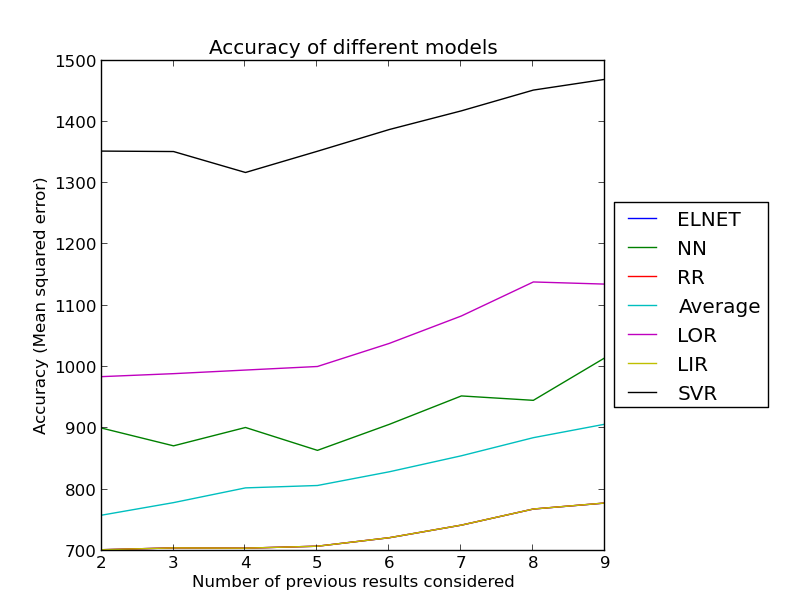
\includegraphics[width=1\textwidth]{images/kfoldall.png}
\caption{Comparison of different machine learning methods comparing their accuracy against the number of previous exercises considered}
\label{fig:kfoldall}
\end{figure}

Figure \ref{fig:kfoldall} appears to tell us that LIR (Linear Regression) performs the best. However, it also seems that RR (Ridge Regression), ELNET (Elastic Net) and Lasso are missing from the graph. However, if the graph is magnified on the Linear Regression line we get Figure \ref{fig:zoomed}

\begin{figure}[p]
\centering
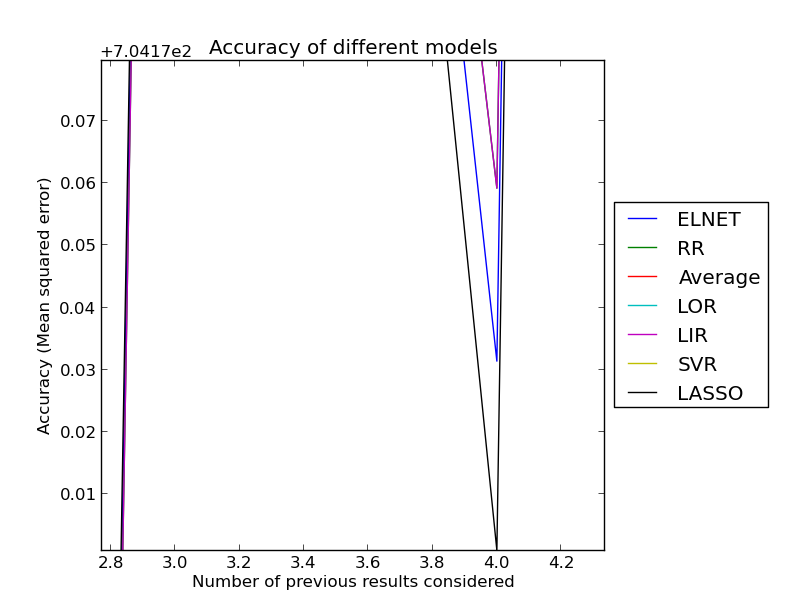
\includegraphics[width=1\textwidth]{images/linearmodels.png}
\caption{Similarity of the linear models}
\label{fig:zoomed}
\end{figure}

This graph shows that the linear models all perform very similarly with their maximum variance being displayed in Figure \ref{fig:zoomed} as roughly 0.06. Although not visible in the previous figure, it can be seen in Figure \ref{fig:whereisrr} that Ridge Regression follows Linear Regression very closely.

\begin{figure}[p]
\centering
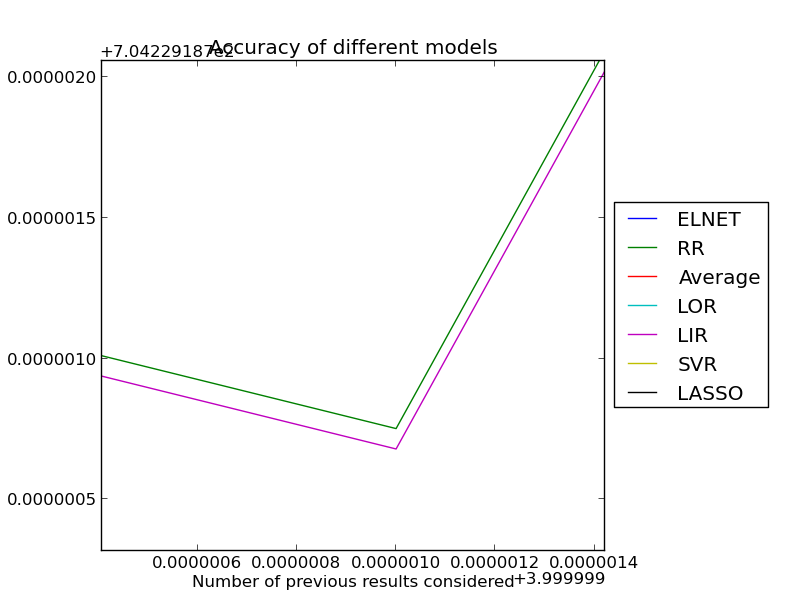
\includegraphics[width=1\textwidth]{images/whereisrr.png}
\caption{Ridge regression follows extremely closely to linear regression}
\label{fig:whereisrr}
\end{figure}


\section{Final model}

\subsection{Optimisation}

\section{Testing the model}
